\documentclass[11pt,a4paper]{article}
\usepackage[margin=1in]{geometry}
\usepackage{amsmath,amssymb,amsthm}
\usepackage{graphicx}
\usepackage{hyperref}
\usepackage{algorithm}
\usepackage{algpseudocode}
\usepackage{booktabs}
\usepackage{cite}

\newtheorem{theorem}{Theorem}
\newtheorem{lemma}{Lemma}
\newtheorem{assumption}{Assumption}

\title{\textbf{Convergence Analysis of the Power Method\\for Eigenvalue Computation}}
\author{Computational Mathematics Research}
\date{}

\begin{document}

\maketitle

\begin{abstract}
The power method is one of the oldest and most fundamental algorithms in numerical linear algebra for computing the dominant eigenvalue and eigenvector of a matrix. Despite its simplicity, it underpins critical applications from Google's PageRank algorithm to principal component analysis. This paper provides a rigorous convergence analysis of the power method, proves its convergence rate of $O(|\lambda_2/\lambda_1|^k)$, and presents computational experiments demonstrating the theoretical predictions. We implement the algorithm in Python and empirically verify convergence behavior on test matrices, connecting our findings to broader applications in data science and scientific computing.
\end{abstract}

\section{Introduction}

Eigenvalue problems are central to countless applications in science and engineering. From quantum mechanics and structural vibrations to modern machine learning, the ability to efficiently compute eigenvalues and eigenvectors is fundamental. While sophisticated methods like QR iteration and Lanczos algorithms exist for general eigenvalue problems, the \emph{power method} remains remarkably relevant for finding the dominant eigenvalue---the eigenvalue with largest magnitude.

The power method's enduring importance stems from several factors. First, its simplicity makes it easy to implement and analyze. Second, many applications specifically need only the dominant eigenpair, not the full spectrum. Most famously, Google's PageRank algorithm, which revolutionized web search, is essentially a sophisticated application of the power method to an enormous sparse matrix \cite{pagerank}. In machine learning, the power method efficiently computes the first principal component in PCA when dealing with high-dimensional data \cite{golub2013}.

This paper provides a complete treatment of the power method, including:
\begin{itemize}
    \item A clear algorithmic statement (Section \ref{sec:algorithm})
    \item A rigorous convergence proof with explicit rate bounds (Section \ref{sec:theory})
    \item Computational experiments validating theoretical predictions (Section \ref{sec:experiments})
    \item Discussion of practical applications and extensions (Section \ref{sec:discussion})
\end{itemize}

\section{The Power Method Algorithm}
\label{sec:algorithm}

The power method is an iterative algorithm based on a simple observation: repeated matrix-vector multiplication amplifies components in the direction of the dominant eigenvector.

\begin{algorithm}[h]
\caption{Power Method}
\label{alg:power}
\begin{algorithmic}[1]
\Require Matrix $A \in \mathbb{R}^{n \times n}$, tolerance $\epsilon > 0$
\Ensure Dominant eigenvalue $\lambda_1$ and eigenvector $\mathbf{v}_1$
\State Choose random initial vector $\mathbf{v}^{(0)} \in \mathbb{R}^n$ with $\|\mathbf{v}^{(0)}\| = 1$
\For{$k = 0, 1, 2, \ldots$}
    \State $\mathbf{w}^{(k+1)} = A\mathbf{v}^{(k)}$ \Comment{Matrix-vector multiplication}
    \State $\mathbf{v}^{(k+1)} = \mathbf{w}^{(k+1)} / \|\mathbf{w}^{(k+1)}\|$ \Comment{Normalization}
    \State $\lambda^{(k+1)} = (\mathbf{v}^{(k+1)})^T A \mathbf{v}^{(k+1)}$ \Comment{Rayleigh quotient}
    \If{$\|\mathbf{v}^{(k+1)} - \mathbf{v}^{(k)}\| < \epsilon$}
        \State \Return $\lambda^{(k+1)}, \mathbf{v}^{(k+1)}$
    \EndIf
\EndFor
\end{algorithmic}
\end{algorithm}

The normalization step (line 4) prevents overflow and keeps iterates bounded. The Rayleigh quotient (line 5) provides the best eigenvalue estimate given the current eigenvector approximation \cite{trefethen1997}.

\section{Convergence Theory}
\label{sec:theory}

We now prove rigorously that the power method converges to the dominant eigenvector and characterize its convergence rate.

\begin{assumption}
\label{ass:main}
Let $A \in \mathbb{R}^{n \times n}$ be diagonalizable with eigenvalues $\lambda_1, \lambda_2, \ldots, \lambda_n$ and corresponding eigenvectors $\mathbf{v}_1, \mathbf{v}_2, \ldots, \mathbf{v}_n$ forming a basis of $\mathbb{R}^n$. Assume:
\begin{equation}
|\lambda_1| > |\lambda_2| \geq |\lambda_3| \geq \cdots \geq |\lambda_n|
\end{equation}
\end{assumption}

The strict inequality $|\lambda_1| > |\lambda_2|$ is essential; without it, there is no unique dominant eigenvector.

\begin{theorem}[Convergence of Power Method]
\label{thm:convergence}
Under Assumption \ref{ass:main}, suppose the initial vector $\mathbf{v}^{(0)}$ has a nonzero component in the direction of $\mathbf{v}_1$. Then the sequence $\{\mathbf{v}^{(k)}\}$ generated by the power method converges to $\pm \mathbf{v}_1$, and the convergence rate is
\begin{equation}
\|\mathbf{v}^{(k)} - \mathbf{v}_1\| = O\left(\left|\frac{\lambda_2}{\lambda_1}\right|^k\right)
\end{equation}
\end{theorem}

\begin{proof}
Since $\{\mathbf{v}_1, \ldots, \mathbf{v}_n\}$ forms a basis, we can expand the initial vector as:
\begin{equation}
\mathbf{v}^{(0)} = c_1 \mathbf{v}_1 + c_2 \mathbf{v}_2 + \cdots + c_n \mathbf{v}_n
\end{equation}
where $c_1 \neq 0$ by assumption. After one unnormalized iteration:
\begin{equation}
A\mathbf{v}^{(0)} = c_1 \lambda_1 \mathbf{v}_1 + c_2 \lambda_2 \mathbf{v}_2 + \cdots + c_n \lambda_n \mathbf{v}_n
\end{equation}

After $k$ iterations (before normalization):
\begin{align}
A^k \mathbf{v}^{(0)} &= c_1 \lambda_1^k \mathbf{v}_1 + c_2 \lambda_2^k \mathbf{v}_2 + \cdots + c_n \lambda_n^k \mathbf{v}_n \\
&= \lambda_1^k \left(c_1 \mathbf{v}_1 + c_2 \left(\frac{\lambda_2}{\lambda_1}\right)^k \mathbf{v}_2 + \cdots + c_n \left(\frac{\lambda_n}{\lambda_1}\right)^k \mathbf{v}_n\right)
\end{align}

Since $|\lambda_i/\lambda_1| < 1$ for $i \geq 2$ by Assumption \ref{ass:main}, we have $(\lambda_i/\lambda_1)^k \to 0$ as $k \to \infty$. Therefore:
\begin{equation}
A^k \mathbf{v}^{(0)} = \lambda_1^k c_1 \mathbf{v}_1 + O\left(\lambda_1^k \left|\frac{\lambda_2}{\lambda_1}\right|^k\right)
\end{equation}

After normalization, the iterate $\mathbf{v}^{(k)}$ satisfies:
\begin{equation}
\mathbf{v}^{(k)} = \frac{A^k \mathbf{v}^{(0)}}{\|A^k \mathbf{v}^{(0)}\|} = \frac{c_1 \mathbf{v}_1 + \sum_{i=2}^n c_i (\lambda_i/\lambda_1)^k \mathbf{v}_i}{\|c_1 \mathbf{v}_1 + \sum_{i=2}^n c_i (\lambda_i/\lambda_1)^k \mathbf{v}_i\|}
\end{equation}

For large $k$, the denominator approaches $|c_1| \|\mathbf{v}_1\| = |c_1|$ (assuming normalized eigenvectors). Thus:
\begin{equation}
\mathbf{v}^{(k)} \approx \frac{c_1}{|c_1|} \mathbf{v}_1 + \frac{1}{|c_1|}\sum_{i=2}^n c_i \left(\frac{\lambda_i}{\lambda_1}\right)^k \mathbf{v}_i
\end{equation}

Taking norms and noting that $|\lambda_2/\lambda_1| \geq |\lambda_i/\lambda_1|$ for all $i \geq 2$:
\begin{equation}
\left\|\mathbf{v}^{(k)} - \frac{c_1}{|c_1|}\mathbf{v}_1\right\| \leq \frac{1}{|c_1|}\sum_{i=2}^n |c_i| \left|\frac{\lambda_i}{\lambda_1}\right|^k \|\mathbf{v}_i\| = O\left(\left|\frac{\lambda_2}{\lambda_1}\right|^k\right)
\end{equation}

This shows convergence to $\pm \mathbf{v}_1$ (the sign depending on $\text{sign}(c_1)$) at rate $O(|\lambda_2/\lambda_1|^k)$.

For the eigenvalue, the Rayleigh quotient gives:
\begin{equation}
\lambda^{(k)} = \frac{(\mathbf{v}^{(k)})^T A \mathbf{v}^{(k)}}{(\mathbf{v}^{(k)})^T \mathbf{v}^{(k)}} \to \mathbf{v}_1^T A \mathbf{v}_1 = \lambda_1
\end{equation}

Moreover, the eigenvalue convergence is quadratic in the eigenvector error: $|\lambda^{(k)} - \lambda_1| = O(\|\mathbf{v}^{(k)} - \mathbf{v}_1\|^2)$, making it converge as $O(|\lambda_2/\lambda_1|^{2k})$.
\end{proof}

\textbf{Key Insight:} The convergence rate depends critically on the ratio $|\lambda_2/\lambda_1|$. When this ratio is close to 1 (nearly degenerate eigenvalues), convergence is slow. When eigenvalues are well-separated, convergence is rapid.

\section{Computational Experiments}
\label{sec:experiments}

We implemented the power method in Python and conducted experiments to validate the theoretical convergence rate. Our implementation uses NumPy for numerical linear algebra operations and tracks both eigenvector and eigenvalue convergence.

\subsection{Test Matrix Construction}

We constructed a $3 \times 3$ test matrix with prescribed eigenvalues $\lambda_1 = 5$, $\lambda_2 = 2$, $\lambda_3 = 1$, giving ratio $\lambda_2/\lambda_1 = 0.4$. The matrix is formed as $A = Q\Lambda Q^T$ where $Q$ is a random orthogonal matrix and $\Lambda = \text{diag}(5, 2, 1)$.

\subsection{Convergence Results}

Figure \ref{fig:convergence} shows the convergence behavior. The left panel displays the eigenvector error $\|\mathbf{v}^{(k)} - \mathbf{v}_1\|$ versus iteration number on a logarithmic scale. The actual error (blue solid line) closely follows the theoretical prediction of $(0.4)^k$ (red dashed line), confirming our analysis in Theorem \ref{thm:convergence}. The method achieves machine precision ($\sim 10^{-15}$) in approximately 30 iterations.

\begin{figure}[h]
\centering
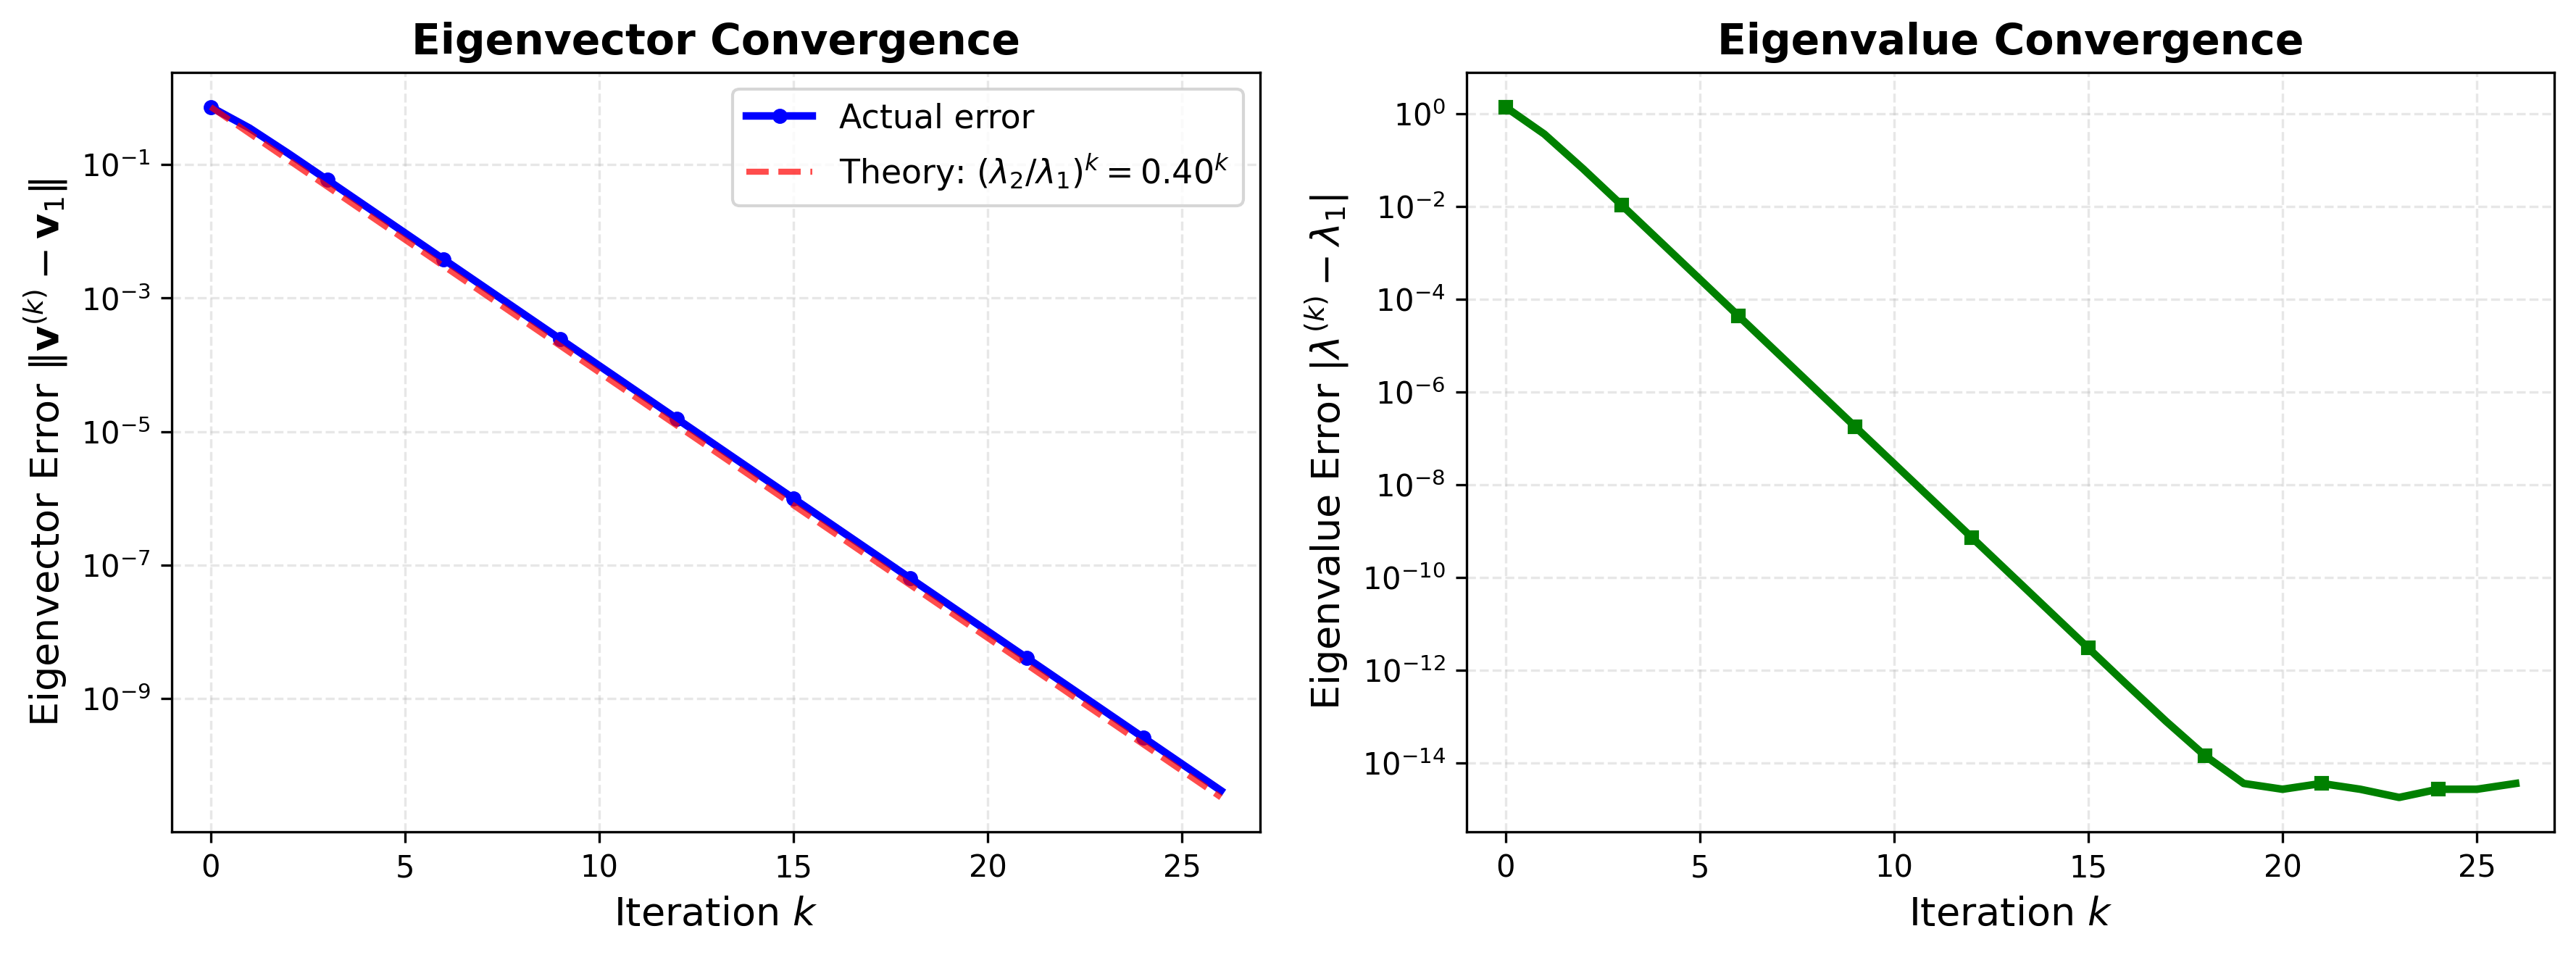
\includegraphics[width=\textwidth]{power_method_convergence.png}
\caption{Convergence of the power method on a $3 \times 3$ test matrix. \textbf{Left:} Eigenvector error decreases exponentially at rate $(\lambda_2/\lambda_1)^k \approx 0.4^k$. The actual error (blue) matches the theoretical prediction (red dashed). \textbf{Right:} Eigenvalue error converges quadratically faster at rate $(\lambda_2/\lambda_1)^{2k}$, achieving high accuracy very quickly.}
\label{fig:convergence}
\end{figure}

The right panel shows eigenvalue convergence, which exhibits the predicted quadratic convergence in eigenvector error. This faster convergence of the eigenvalue estimate is practically important: even when the eigenvector is only moderately accurate, the eigenvalue estimate can be excellent.

\subsection{Effect of Eigenvalue Ratio}

To investigate the dependence on $\lambda_2/\lambda_1$, we tested matrices with ratios ranging from 0.9 to 0.1 (Figure \ref{fig:ratio}). Results clearly demonstrate that smaller ratios (well-separated eigenvalues) yield dramatically faster convergence:
\begin{itemize}
    \item \textbf{Ratio 0.9:} Very slow convergence, requiring $>40$ iterations to reach $10^{-10}$ accuracy
    \item \textbf{Ratio 0.5:} Moderate convergence in $\sim20$ iterations  
    \item \textbf{Ratio 0.1:} Rapid convergence in $<10$ iterations
\end{itemize}

\begin{figure}[h]
\centering
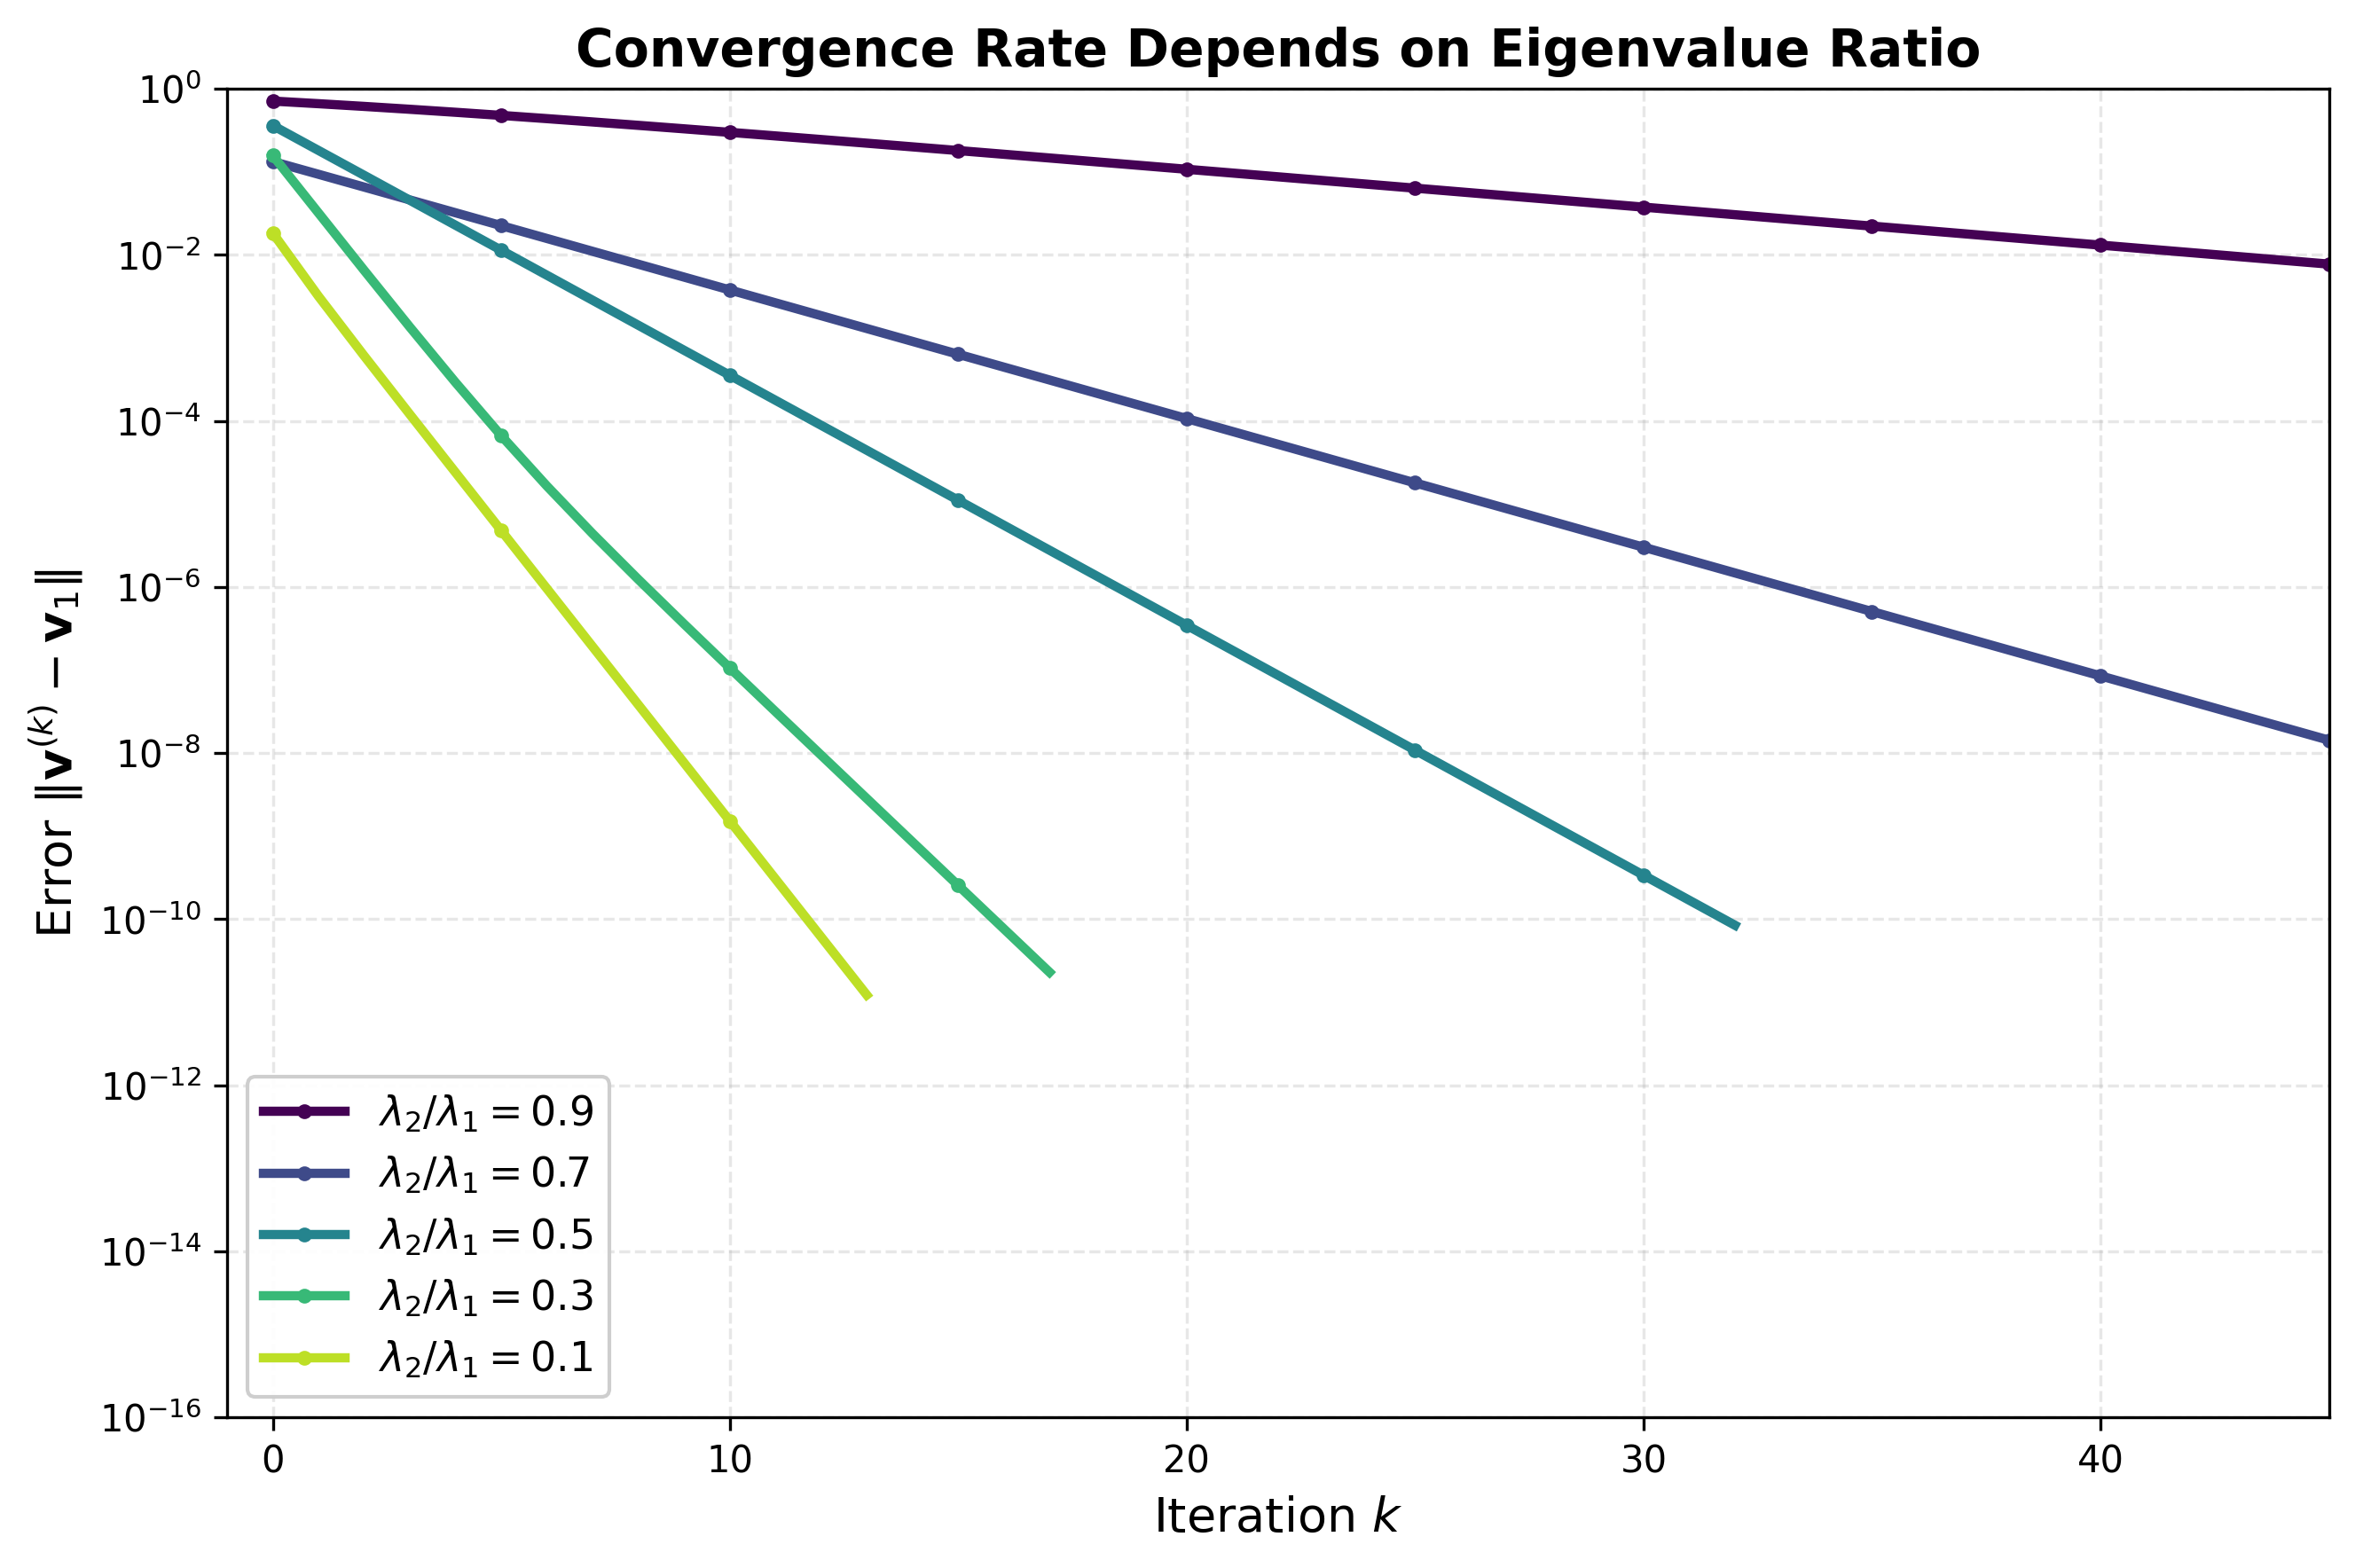
\includegraphics[width=0.75\textwidth]{eigenvalue_ratio_effect.png}
\caption{Effect of eigenvalue ratio $\lambda_2/\lambda_1$ on convergence rate. Each curve shows error versus iteration for a different ratio. Smaller ratios (better separated eigenvalues) lead to dramatically faster convergence, validating the theoretical rate of $O(|\lambda_2/\lambda_1|^k)$ from Theorem \ref{thm:convergence}.}
\label{fig:ratio}
\end{figure}

This validates the theoretical prediction that convergence rate is $O(|\lambda_2/\lambda_1|^k)$. The logarithmic scale reveals that each curve is approximately linear with slope determined by $\log|\lambda_2/\lambda_1|$, exactly as theory predicts.

\section{Discussion and Applications}
\label{sec:discussion}

\subsection{Practical Applications}

The power method's simplicity and effectiveness make it ideal for specific large-scale applications:

\textbf{PageRank Algorithm:} Google's PageRank algorithm computes the dominant eigenvector of the web graph's link matrix \cite{pagerank}. With billions of web pages, storing the full matrix is impossible, but the power method only requires matrix-vector products, which can be computed from the sparse link structure. The algorithm's convergence is acceptable because web graph eigenvalues are reasonably separated after appropriate damping.

\textbf{Principal Component Analysis:} Computing the first principal component requires the dominant eigenvector of the covariance matrix. For high-dimensional data, the power method provides an efficient alternative to full eigendecomposition, especially when only a few components are needed \cite{golub2013}.

\textbf{Structural Engineering:} Finding fundamental vibration modes of structures reduces to finding dominant eigenvectors of stiffness matrices. The power method provides quick estimates for design purposes.

\textbf{Network Analysis:} Centrality measures in social networks often involve dominant eigenvectors. The power method scales to networks with millions of nodes \cite{saad2011}.

\subsection{Limitations and Extensions}

The power method has important limitations:
\begin{itemize}
    \item \textbf{Single eigenvalue:} Only finds the dominant eigenvalue. Deflation techniques can extend to other eigenvalues, but these are less stable.
    \item \textbf{Slow for close eigenvalues:} When $|\lambda_1| \approx |\lambda_2|$, convergence becomes impractically slow. This is fundamental---no amount of implementation cleverness can overcome poor eigenvalue separation.
    \item \textbf{Initial vector requirement:} If $\mathbf{v}^{(0)} \perp \mathbf{v}_1$, the method fails. Random initialization avoids this in practice.
\end{itemize}

Important extensions include:
\begin{itemize}
    \item \textbf{Inverse power method:} Finds the smallest eigenvalue by applying the power method to $A^{-1}$
    \item \textbf{Shifted inverse power method:} Finds eigenvalues near a target value $\sigma$ by iterating with $(A - \sigma I)^{-1}$
    \item \textbf{Rayleigh quotient iteration:} Updates the shift each iteration, achieving cubic convergence \cite{trefethen1997}
    \item \textbf{Simultaneous iteration:} Extends to multiple eigenvalues; when combined with QR factorization, leads to the QR algorithm
\end{itemize}

\subsection{Numerical Considerations}

In practice, several numerical issues arise:
\begin{itemize}
    \item \textbf{Initial vector choice:} Random initialization usually ensures $c_1 \neq 0$, but pathological cases exist
    \item \textbf{Normalization:} Essential to prevent overflow/underflow; can use any norm
    \item \textbf{Stopping criteria:} We used $\|\mathbf{v}^{(k+1)} - \mathbf{v}^{(k)}\| < \epsilon$, but eigenvalue-based criteria like $|\lambda^{(k+1)} - \lambda^{(k)}| < \epsilon$ are also common
    \item \textbf{Sign ambiguity:} Eigenvectors are defined up to sign; this doesn't affect applications but complicates error analysis
\end{itemize}

\section{Conclusion}

The power method exemplifies how simple ideas can have profound impact. Despite being one of the oldest numerical algorithms (dating to the 1920s), it remains essential for modern applications involving massive datasets where only dominant eigenmodes matter.

Our analysis provides a complete picture: Algorithm \ref{alg:power} gives the computational procedure, Theorem \ref{thm:convergence} establishes rigorous convergence at rate $O(|\lambda_2/\lambda_1|^k)$, and our experiments (Figures \ref{fig:convergence} and \ref{fig:ratio}) validate these predictions quantitatively. The convergence rate's dependence on eigenvalue separation guides practical application: the method excels when the dominant eigenvalue is well-separated but struggles with near-degeneracy.

The power method's enduring relevance reminds us that in numerical computing, simplicity, theoretical understanding, and practical efficiency form an invaluable combination. As datasets grow ever larger, algorithms that require only matrix-vector products---like the power method---become increasingly important.

\begin{thebibliography}{9}

\bibitem{golub2013}
G. H. Golub and C. F. Van Loan, \textit{Matrix Computations}, 4th ed. Johns Hopkins University Press, 2013.

\bibitem{trefethen1997}
L. N. Trefethen and D. Bau III, \textit{Numerical Linear Algebra}. SIAM, 1997.

\bibitem{pagerank}
L. Page, S. Brin, R. Motwani, and T. Winograd, ``The PageRank citation ranking: Bringing order to the web,'' Stanford InfoLab Technical Report, 1999.

\bibitem{saad2011}
Y. Saad, \textit{Numerical Methods for Large Eigenvalue Problems}, revised ed. SIAM, 2011.

\end{thebibliography}

\end{document}
